\documentclass[a4paper]{article}
\title{\textcolor{red}{Workshop on Public Key Infrastructure and Red Hat Certificate System}}
\author{Niranjan M.R}
\date{}
\usepackage{color}
\usepackage{graphics}
\usepackage{graphicx,subfig}
\begin{document}
\maketitle
\tableofcontents
\section{Introduction to Public Key Cryptography}
Before we start discussing about public key cryptography, we will in general discuss about how system communicate
and what are the various threat models that are associated with the communication medium and what are the tools to 
overcome them.

\textbf{Example1:}
The most common protocol used to communicate between 2 systems is TCP/IP. TCP/IP allows information to be sent 
from one system to another system directly or through many intermediate systems.

Below are some of the threat models associated with above communcation:
\begin{itemize}
    \item \textbf{Eavesdropping:}
        
        Information remains intact, But it's privacy is compromised, For example: some one could learn credit card number, record a sensitive conversation or intercept a
        classified information.
    \item \textbf{Tampering:}

        Information in transit is changed or replaced and then sent to the recipient. For example: Some one could alter an order of goods or change a persons resume.
    \item \textbf{Impersonation:}

        Information passes to a person who poses as intended recipient. Impersonation can take 2 forms:
    \begin{itemize}
        \item \textbf{Spoofing:}

            A person can pretend to be someone else, For example, a person can pretend to have email address \textit{joe@example.net}, 
            or computer can identify itself as a site called www.example.net, when it is not. This type of impersonation is called spoofing.
        \item \textbf{Misrepresentation:}

            A person or organization can misrepresent itself, For example, suppose the site \textit{www.example.net} pretends to be a 
            furniture store when it's just a site which accepts payments but never sends any goods.
    \end{itemize}
\end{itemize}
\textbf{Example2:}
Consider Alice , Bob and attacker are the parties , where alice and bob want to communicate to each other and Attacker is a threat to the communication.

\begin{itemize}
    \item Alice can send a postcard to bob to communicate, but this method is very weak as any random eavesdropper could read the postcard.
    \item Alice could write a letter and put in an envelope and send it to bob, but the attacker could open the envelope and read the letter, 
        both confidentiality and integrity of the message is lost.
    \item Alice could seal the envelope with wax , but this method too is inefficient as Attacker could read the letter and seal it as it is 
        without bob knowing that it was read by attacker
    \item Alice could write a letter and put it in a safe which has 2 keys and send one key before to Bob , and send the safe across to bob, 
        this ensures confidentiality, integrity but practically this is not implementable. Considering the number of 
        messages that has to be transferred , it's impractical to implement the mail safe method.
\end{itemize}

To mitigate above threat models, we will look in to cryptology as one of the tools of the trade. 

\textbf{Cryptology:} Cryptology is the theory of designing the various algorithms we use to provide security

\textbf{Cryptography:} Cryptography is the study of using these algorithms to secure systems and protocols.
\subsection{Encryption}
An encryption algorithm takes some data(called plaintext) and converts it to cipher-text under control of a key. 
cipher text contains random data which makes no sense without the key.  

A key is a short random string (8-24 bytes): 

\begin{picture}(10,10)(10,10)
    \put(40,1){\framebox(55,8){Plain Text}} 
    \put(102,10){\tiny Encryption}
    \put(102,4){\vector(1,0){30}}
    \put(140,1){\framebox(55,8){Cipher Text}} 
    \put(200,10){\tiny Decryption}
    \put(200,4){\vector(1,0){30}}
    \put(240,1){\framebox(55,8){Plain Text}} 
\end{picture}
\linebreak

When a message is encrypted and received , we cannot say if it's not tampered with. An encryption is strong when 
it can determine the number of possible keys. The attacker tries each key one at a time until he finds a key that 
produces a plausible decryption. The security of the algorithm should solely depend on the secrecy of the key. 
The algorithm should not need to be secret.

If the attacker knows the plaintext corresponding to the ciphertext it's called \textit{``known plaintext attack''} .

An attack where attacker doesn't know the plaintext , it's called \textit{``ciphertext-only attack''}.
\textit{Ex:} If the attacker knows that plaintext is ASCII , so any decryption which uses non-ascii characters must be using the wrong key.
\subsubsection{Symmetric Encryption}
When Sender and recipient share the same key(which must be kept secret) is referred to as \textit{Symmetric Key Cryptograph} or also
referred to as \textit{Secret Key Cryptography} as opposed to \textit{Public Key Cryptography}citation required?.
\begin{figure}[h]
    \centering
    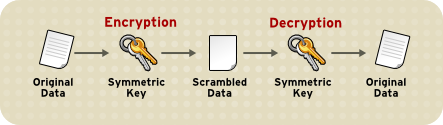
\includegraphics[width=50mm]{symmetric.png}
    \caption{Symmetric Encryption}
\end{figure}
\subsubsection{Assymetric Encryption}
\begin{itemize}
    \item First started in stanford university by Whitfield Diffie and Martin Hellman
    \item The most commonly used implementation of PKC are based on algorithm based on algorithm patented by RSA data security.
    \item Each public key is published \& private key is kept secret. Data encrypted with public key can be decrypted only with private key.
    \item In general, to send encrypted data to someone, we encrypt with public key \& the person encrypt receiving the 
        encrypted data decrypts with private key
    \item Compared to symmetric key encryption, public key encryption requires more computation \& therefore not always appropriate for large amounts of data
    \item It is possible to use public-key encryption to send a symmetric key, which can then be used to encrypt additional data.
        \begin{figure}[h]
        \centering
        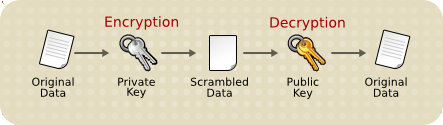
\includegraphics[width=80mm]{assymetric.png}
        \caption{Assymetric Encryption}
    \end{figure}
    \item Reverse of the above figure also happens i.e. encrypt with private key and decrypt with public-key. But not useful for sensitive information
        \begin{figure}[h]
        \centering
        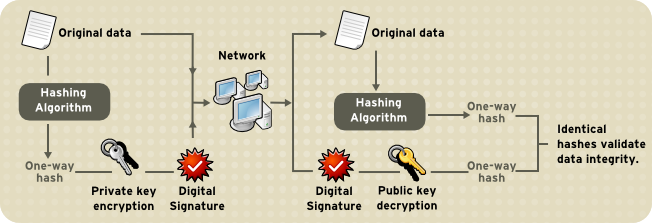
\includegraphics[width=80mm]{digitalsignature.png}
        \caption{Digital Signature}
        \end{figure}
    \item There's a problem with the above method, how would the parties get each other's public-key ? 
        If we send the keys through electronically, then the attacker an tamper, while they are in transit to the receiver.
    \item When the 2 parties want to communicate, the attacker can intercept the keys \& instead send his own key to each other, 
        thus each party encrypts to him and \& he re-encrypts it to the real recipient. 
        This is called \textit{man-in-the-middle attack}
        \begin{figure}[ht!]
            \centering
            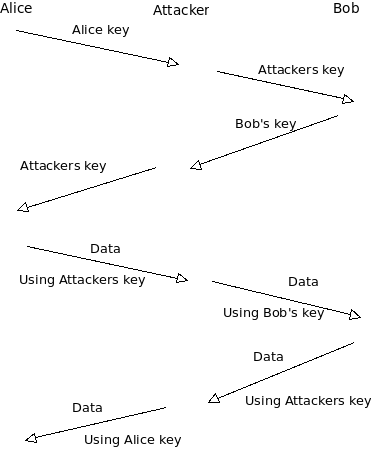
\includegraphics[width=50mm]{mitm.png}
            \caption{Man-in-the-middle attack}
        \end{figure}
\end{itemize}
\subsection{Message Digest}
A message digest is simply a function that takes as an input an arbitrary message and outputs a fixed length string 
which is characteristic of the message. The important property here is irreversibility.  
It's extremely difficult to compute a message from the given digest. 
Property of the message digest: 
\begin{itemize}
    \item For a digest to be secure, it must be difficult to generate any of the message that digests to the same value. 
        You have to search a message space of proportional size of the digest in order to find a matching message text
    \item It should be difficult to produce 2 messages M and M' such that they have the same digest. 
        This property is called collision-resistance. It turns out that the strength of any message digest 
        against finding collision is only half the size of the digest., so a 128-bit digest is only 64 bits strong against collisions.
\end{itemize}
\subsubsection{Message Authentication Code}
Consider \textit{Alice} and \textit{Bob} share a key and Alice wants to send a message to \textit{Bob}. The message can be encrypted, 
and send it across to \textit{Bob}, but we are not sure that the encrypted message would be tampered and also not sure 
if \textit{Alice} was the one who sent the encrypted message.  So we use a new tool called \textit{MAC} . \textit{MAC} is a digest algorithm,
but with a key, So the MAC is dependent on both the key and the message being MACed.
\subsection{Protocols}
\subsection{Exercises}
\section{Introduction to Public Key Infrastructure}
\subsection{Common Terms used in PKI}
\subsection{Detailed look on certificate/CRL}
\subsection{Exercises}
\section{Red Hat Certificate System}
\subsection{Certificate Manager}
\subsubsection{Introduction}
Certificate Manager is the first subsystem that needs to be configured in PKI Environment, Certificate Manager can be configured as RootCA, Subordinate CA
\subsubsection{Key Features}
    \begin{itemize}
        \item CA subsystem issues, renews, revokes Certificates, generates Certificat Revocation lists
        \item Publishes Certificates/CRL in form of files or can publish to LDAP or OCSP responder
        \item CA also has an inbuilt OCSP responder enabling OCSP-Compliant clients to query CA about revocation status of Certificate
        \item Some CA's can delegate some of it's responsibility to another Subordinate CA
    \end{itemize}
\subsubsection{Architecture}
     \begin{figure}[ht!]
          \centering
          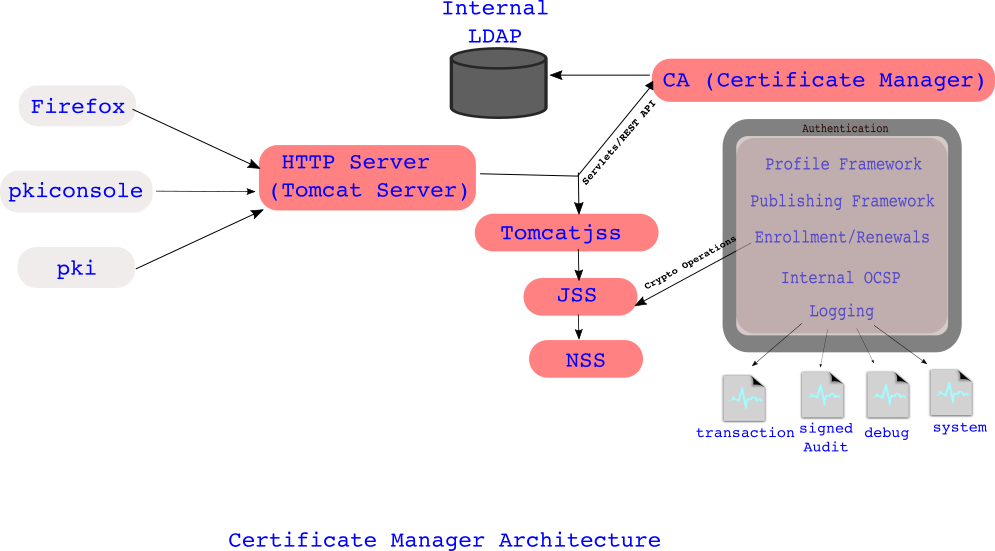
\includegraphics[width=120mm]{CA-subsystem-Arch3.png}
          \caption{CA Subsystem Architecture}
    \end{figure}
\subsubsection{Interfaces}
    \begin{itemize}
        \item End User Interface(Browser/CLI)
        \item Agent Interface(Browser/CLI)
        \item Admin interface(java console)
    \end{itemize}
\subsubsection{Features}
\subsubsection{Exercises}
\subsection{Key Recovery Authority}
\subsection{Online Certificate Status Protocol}
\subsection{Token Key Service \& Token Processing System}
\end{document}
